\documentclass[12pt]{article}
\usepackage{amsmath, amssymb}
\usepackage[margin=1in]{geometry}
\usepackage{hyperref}
\usepackage{enumitem}
\usepackage{siunitx}
\usepackage{xcolor}
\usepackage[dvipsnames]{xcolor}
\usepackage{lscape}
\usepackage{tikz}
\usetikzlibrary{arrows.meta}
\usetikzlibrary{decorations.markings}
\usetikzlibrary{patterns}
\usetikzlibrary{positioning,arrows}
\usetikzlibrary{decorations.pathmorphing}
\usetikzlibrary{shapes.multipart}


\usepackage{titlesec}
\titlelabel{\thetitle.~}

\usepackage{fancyhdr}
\pagestyle{fancy}
\renewcommand{\headrulewidth}{0pt}
\fancyhf{}

\usepackage{lastpage}
\setlength\headheight{15pt}

\usepackage{multirow}

\usepackage{siunitx}


\begin{document}

\lfoot{\footnotesize UCSB Physics Instructional Lab Group. Last Revision: 04/22/2026.}
\rfoot{\small page \thepage~of \pageref{LastPage}}

\hfil {\large University of California, Santa Barbara} \hfil

\vspace{0.1in}

\hfil {\large Department of Physics}\hfil

\normalfont

\begin{center}
    \LARGE \bfseries
    Physics 20CL\\
    The Spectrum of Atomic Hydrogen Test 2
\end{center}

\textbf{Objective}: the goal of this experiment is to accurately measure the wavelength of the first four visible hydrogen emission spectral lines in the Balmer series using a grating spectroscope. The Rydberg constant for hydrogen is calculated and compared to the accepted value. This measurement is crucial to the understanding and development of quantum physics.

\textbf{Materials}: student spectroscope, diffraction grating (600 l/mm) in its mount, gas-discharge tubes, power supply, auxiliary white light source with an eyepiece attachment, protected aluminum mirror in its mount, spirit level.

\vspace{0.3in}

\hfil \textbf{\Large THEORY} \hfil

\vspace{-0.1in}

\section{The Hydrogen Spectrum}
The hydrogen atom is the simplest atomic system consisting of a single electron and a single proton interacting via the attractive Coulomb potential. A distinct feature of such bound microscopic system is the existence of discrete energy levels, or states. Transitions between these states can occur in which an isolated system decays spontaneously to a lower state, emitting a quantum of radiation (a photon). In the presence of an external field, the system can either lose energy to the field, emitting a photon, or gain energy from it, absorbing a~photon.

These transitions are fundamental differences between quantum physics and classical physics. 

In the nineteenth century it was found that hot atomic gases emit and absorb light only at certain frequencies, or wavelengths, and that the pattern of frequencies, called a spectrum, was characteristic of the atomic element that makes up the gas. Kirchhoff and Bunsen identified two new elements, cesium and rubidium, by their distinctive emission spectra, establishing spectroscopy as a powerful tool for chemical analysis. Forty years prior Fraunhofer observed dark lines in the spectrum of the Sun found to be the result of absorption of light in its cooler outer layers.

Early attempts to explain regularities in the observed pattern of spectral line frequencies led to an empirical discovery by Balmer, who found that the series of emission lines in the spectrum of hydrogen are very accurately described by the simple formula:
\begin{equation}\label{Balmer}
    \frac{1}{\lambda} = R \left(\frac{1}{2^2}-\frac{1}{m^2}\right); \quad m=1,2,\dots
\end{equation}
where $\lambda$ is the wavelength of the spectral line, $R$ is a constant and $m$ is an integer. Balmer's formula is a special case of a more general empirical relation $1/\lambda = R \left(1/n^2-1/m^2\right)$ discovered by Rydberg who studied the spectral lines of many elements, notably those of the alkali metals.

Although the physical meaning of Balmer's formula was not understood at the time, it correctly described the spectrum of hydrogen from the far ultra-violet to the infra-red. The fact that the frequency of spectral lines can be expressed as the difference between the two ``terms" in the parentheses of Eqn.~(\ref{Balmer}) was later generalized to the \textit{Rydberg--Ritz combination principle}, from which \textit{other} lines in the same spectrum could be identified by taking \textit{differences} of the known terms.

The first successful attempt to explain the hydrogen spectrum was due to Bohr. Bohr and Sommerfeld established the foundations of what is now referred to as the ``old" quantum theory. This theory correctly accounted for both the existence of sharp spectral lines and the Rydberg--Ritz combination principle.

The first of Bohr's postulates asserts that of all the states allowed by the laws of classical mechanics only certain discrete, \textit{stationary} states are permitted. In contrast to the rules of classical electrodynamics, a charged electron does \textit{not} radiate energy while the atom is in a stationary state. The emission or absorption of energy occurs when an atom \textit{transitions} from one stationary state to another, and the frequencies $\nu_{n,m}$ of emission and absorption of light are related, according to the second postulate, to the corresponding energies $E_n$ and~$E_m$ of the stationary states: 
\begin{equation}\label{Bohr_frequency_relation}
    h \nu_{n,m} = E_n-E_m,
\end{equation}
where $h$ is the \href{https://www.nist.gov/physics/explainers/planck-constant}{Planck constant}.  The link is to the NIST (National Institute of Standards and Technology) web page.  One of the challenges in doing quantum physics is mastering the constants and the units.

\begin{figure}[ht!]
    \centering
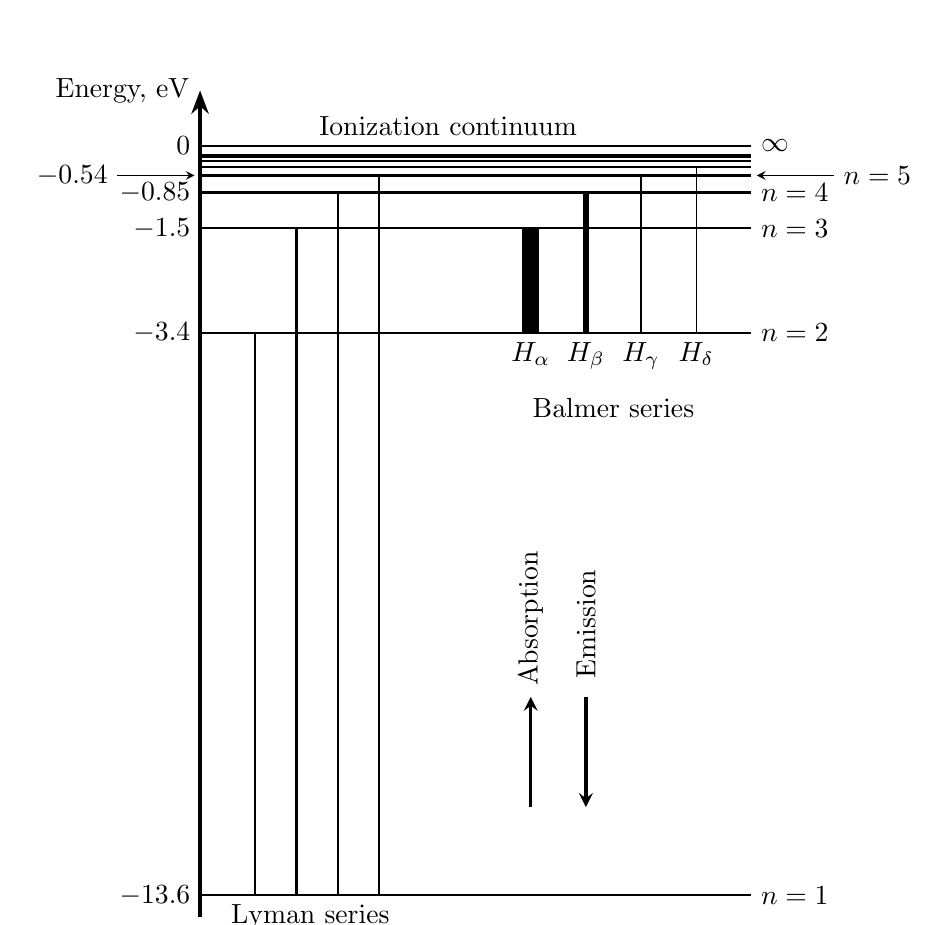
\begin{tikzpicture}[scale=0.7]
\foreach \x in {-13.6,-3.4,-1.5,-0.85,-0.54,-0.38,-0.28,-0.21,-0.17,0} {
    \draw[thick] (0,\x) -- (10,\x);
}
\node[left] at (0,-13.6) {$-13.6$}; \node[right] at (10,-13.6) {$n=1$}; \node[left] at (0,-3.4) {$-3.4$}; \node[right] at (10,-3.4) {$n=2$}; \node[left] at (0,-1.5) {$-1.5$}; \node[right] at (10,-1.5) {$n=3$}; \node[left] at (0,-0.85) {$-0.85$}; \node[right] at (10,-0.85) {$n=4$}; \draw[-stealth] (-1.5,-0.54) -- (-0.1,-0.54); \node[left] at (-1.5,-0.54) {$-0.54$}; \node[right] at (11.5,-0.54) {$n=5$}; \draw[-stealth] (11.5,-0.54) -- (10.1,-0.54); \node[left] at (0,0) {$0$}; \node[right] at (10,0) {$\infty$};
\draw[very thick, -Stealth] (0,-14) -- (0,1) node[left] {Energy, eV};

\draw[line width=6pt] (6,-1.5) -- (6,-3.4); 
\draw[line width=2pt] (7,-0.85) -- (7,-3.4);
\draw[line width=0.6pt] (8,-0.54) -- (8,-3.4);
\draw[line width=0.3pt] (9,-0.38) -- (9,-3.4);

\node[below] at (6, -3.4) {$H_{\alpha}$};
\node[below] at (7, -3.4) {$H_{\beta}$};
\node[below] at (8,-3.4) {$H_{\gamma}$};
\node[below] at (9,-3.4) {$H_{\delta}$};


\draw[thick] (1,-3.4) -- (1,-13.6); \draw[thick] (1.75,-1.5) -- (1.75,-13.6); \draw[thick] (2.5,-0.85) -- (2.5,-13.6); \draw[thick] (3.25,-0.54) -- (3.25,-13.6);

\node[below] at (2,-13.6) {Lyman series}; \node[below] at (7.5,-4.4) {Balmer series};
\node[above] at (4.5,0) {Ionization continuum};
\draw[very thick, -stealth] (6,-12) -- (6,-10) node[right, rotate=90] {Absorption};
\draw[very thick, -stealth] (7,-10) -- (7,-12) node[right, rotate=90,xshift=1.5cm] {Emission};

\end{tikzpicture}
    \caption{Spectrum of a hydrogen atom organized into series of lines that share a lower level. The first four transitions in the Lyman and Balmer series are shown. For the Balmer series, the relative intensity of the lines is indicated by their thickness.}
    \label{Hydrogen Spectrum}
\end{figure}

Equipped with Bohr's postulates and the quantization rule permitting only those states for which the angular momentum of the electron in its orbital (classical) motion around the stationary nucleus is equal to an integer multiple of the \emph{reduced} Planck constant ($m_e v r = n \hbar$), the energy of the stationary states of the hydrogen atom are given by (see pre-lab exercise~1):
\begin{equation}\label{Hydrogen_spectrum}
    E_n = -\frac{m_e e^4}{2(4\pi\epsilon_0)^2\hbar^2} \cdot \frac{1}{n^2} \equiv -\text{Ry} \cdot \frac{1}{n^2},
\end{equation}
where the integer $n$ is called \textit{the principal quantum number} of the corresponding state, $m_e$ and $e$ are the mass and the charge of the electron, and $\text{Ry = 13.6}$~eV is the Rydberg constant previously denoted as $R$. The factor in parentheses arises because of the choice of SI units. Note that the total energy is negative, indicating that the electron is in a bound~state.

The \href{https://physics.nist.gov/cgi-bin/cuu/Value?hbar}{reduced Planck constant} is $\hbar=h/(2\pi)$.  The units can keep you off balance!  Sorry about that! Pesky factors of $\pi$ come and go, as you know from electromagnetism.

The Bohr frequency relation Eqn.~(\ref{Bohr_frequency_relation}) can now be rewritten for the energies of the photons emitted in the transitions as:
\begin{equation}\label{photon-energies}
    E_{\gamma} \equiv \frac{hc}{\lambda} = \text{Ry} \left(\frac{1}{n_f^2}-\frac{1}{n_i^2}\right) = 13.6\,\text{eV} \left(\frac{1}{n_f^2}-\frac{1}{n_i^2}\right),
\end{equation}
where $n_i$ and $n_f$ are the principle quantum numbers of the initial and final states, respectively.

As can be seen from Figure \ref{Hydrogen Spectrum}, the spectral lines of hydrogen can be ordered into groups, or \textit{series}, depending on the final state in the transition. In particular, those transitions for which the final state is the ground state of the atom, $n_f=1$, form the \textbf{Lyman series}, with all lines falling in the far ultraviolet part of the spectrum. The \textbf{Balmer series} studied in this experiment corresponds to $n_f=2$ and the first four of its lines fall in the visible part of the spectrum.

The obtained solution Eqn.~(\ref{Hydrogen_spectrum}) for energy states is also valid for any hydrogen-like system, that is, a system with two oppositely charged particles, bound solely by electrostatic forces, such as singly ionized helium, doubly ionized lithium, positronium, etc.

The Rydberg constant calculated for an electron orbiting a \textit{fixed} nucleus is denoted~$R_{\infty}$ and defined via $hc R_{\infty} = \text{Ry}$, where $hc$ is the conversion factor between energy and wavenumber (in units of m$^{-1}$ or cm$^{-1}$). The current accepted value of the Rydberg constant $R_{\infty}$ can be found on the \href{https://physics.nist.gov/cgi-bin/cuu/Value?ryd}{web site} of NIST and is $R_{\infty} = 10 973 731.568 157~\text{m}^{-1}$.

The assumption of an infinitely heavy, stationary nucleus can be dropped by using, instead of the electron mass $m_e$ in Eqn.~(\ref{Hydrogen_spectrum}), the \textit{reduced} mass $\mu = m_e M/(m_e+M)$ of the system comprising the electron and the nucleus, treating the relative motion of the two particles as the motion of a particle with an effective mass $\mu$ in a Coulomb field $-e^2/(4\pi \epsilon_0 r)$. This leads to a measurable \textit{isotopic shift} between e.g. the spectral lines of hydrogen and deuterium (a stable isotope of hydrogen whose nucleus has one proton and one neutron). The corresponding Rydberg constant for Hydrogen is given by:
\begin{equation}
    R_H = R_{\infty} \frac{M}{m_e+M} \simeq R_{\infty} \left( 1- \frac{m_e}{M} \right),
\end{equation}
where the electron-to-proton mass ratio is $m_e/M \simeq 1/1836$.

A full quantum-mechanical treatment of the hydrogen atom shows that the state of the electron in it is described, in general, by \textit{four} quantum numbers: in addition to the principal quantum number $n$, there is an angular momentum quantum number $\ell$ used to define the square of the angular momentum, the magnetic quantum number $m_{\ell}$ having to do with the projection of the angular momentum along a specified axis, and the spin quantum number $m_s$ arising because the electron, in contrast to the point classical particle, possesses an intrinsic angular momentum. These quantum numbers are not independent, and a detailed analysis shows that the energy levels of the hydrogen atom are \textit{degenerate}, that is, for each $n$ there are actually $2n^2$ energy levels. 

It is instructive to rewrite the Bohr energy levels in Eqn.~\ref{Hydrogen_spectrum} using the so-called \textit{fine structure constant} $\alpha = e^2/(4\pi \varepsilon_0 \hbar c) \approx 1/137$. This dimensionless constant plays a fundamental role throughout atomic physics and describes the \textit{strength} of the electromagnetic interactions. The most tightly bound electron (in the state corresponding to the principal quantum number $n = 1$) has energy
\begin{equation}
    E_{n=1} = -\frac{1}{2}\alpha^2 m_e c^2 \approx -\frac{1}{2} \left(\frac{1}{137}\right)^2 0.511~\text{MeV} = -13.6~\text{eV} = -\text{Ry},
    \label{AlphaMe}
\end{equation}
where the rest energy of the electron from Einstein’s famous relationship is $m_e c^2 = 0.511~\text{MeV}$.  The intuitive idea behind Eqn.~\ref{AlphaMe} is that the electromagnetic interaction steals, through an attractive force,  13.6~eV of the near 1/2-million~eV of the electron rest energy.

For the quarks inside neutrons and protons, the strong interaction sucks away essentially \emph{all} of the rest energy.  The resulting physical state of neutrons and protons is both highly relativistic and quantum mechanical.  The math was so hard to devise that it was not until the 1970's that substantial progress occurred.  UCSB Physics faculty member David~Gross shared the 2004 Nobel Prize in Physics for that progress.

The main mode of interaction between the electron and proton in a hydrogen atom is electromagnetic. However, since the electron has an intrinsic angular momentum and is moving relative to the proton, an additional interaction between the electron spin and the proton charge leads to the so-called \textit{spin-orbital interaction}. The associated energy shift due to this coupling is $\alpha^2 \simeq 10^{-4}$ \textbf{times} the energy of the electron. \textit{Relativistic effects} lead to small splittings of the atomic energy levels of \textit{the same order}.

In addition to this \textit{fine structure}, in the spectrum of hydrogen and other atoms a \textit{\textbf{hyper}fine structure} is observed, owing to the interaction between the electron's magnetic moment and the weak magnetic field of the nucleus. Finally, there is the \textit{Lamb shift} related to the very weak interaction of the electron with fluctuations of the electromagnetic field in vacuum, whose observation stimulated the development of quantum electrodynamics.

In order to observe even the fine structure of the hydrogen spectrum, a high-resolution spectrometer is required (see pre-lab exercise 4), and in this lab a treatment based on the old quantum theory and the correction to it due to finite mass of the nucleus are sufficient.

\section{Introduction to Spectroscopy}

A spectro\textit{meter} is a type of optical instrument that allows for the separation of electromagnetic radiation into its monochromatic components and for the measurement of their relative intensities as a function of wavelength, frequency, or energy. In this experiment, you will use a rather old precision instrument called a spectro\textit{scope}, in which the spectrum is observed \textit{visually} through an eyepiece and the intensity of the individual spectral components can only be estimated roughly by eye. 

A typical spectroscope consists of an entrance slit, a collimator with its objective lens, a dispersive element, such as a prism or diffraction grating, and a telescope with an objective lens and an eyepiece (see Figure \ref{Spectroscope}). The dispersive element is positioned on a graduated rotating table (goniometer) and is illuminated by a nearly parallel beam of light formed by the collimator. The source of light (in our experiment, a gas discharge tube) illuminates the entrance slit positioned at the focal plane of the collimator objective. The prism or diffraction grating spatially separates the monochromatic constituents of the incident radiation into a spectrum. The image of this spectrum is formed in the focal plane of the telescope objective and is viewed by means of the eyepiece focused on the cross hairs which provide a relative reference. Each spectral line is imaged into a diffraction image of the entrance slit (recall the Diffraction Lab!).

\begin{figure}[ht!]
    \centering
    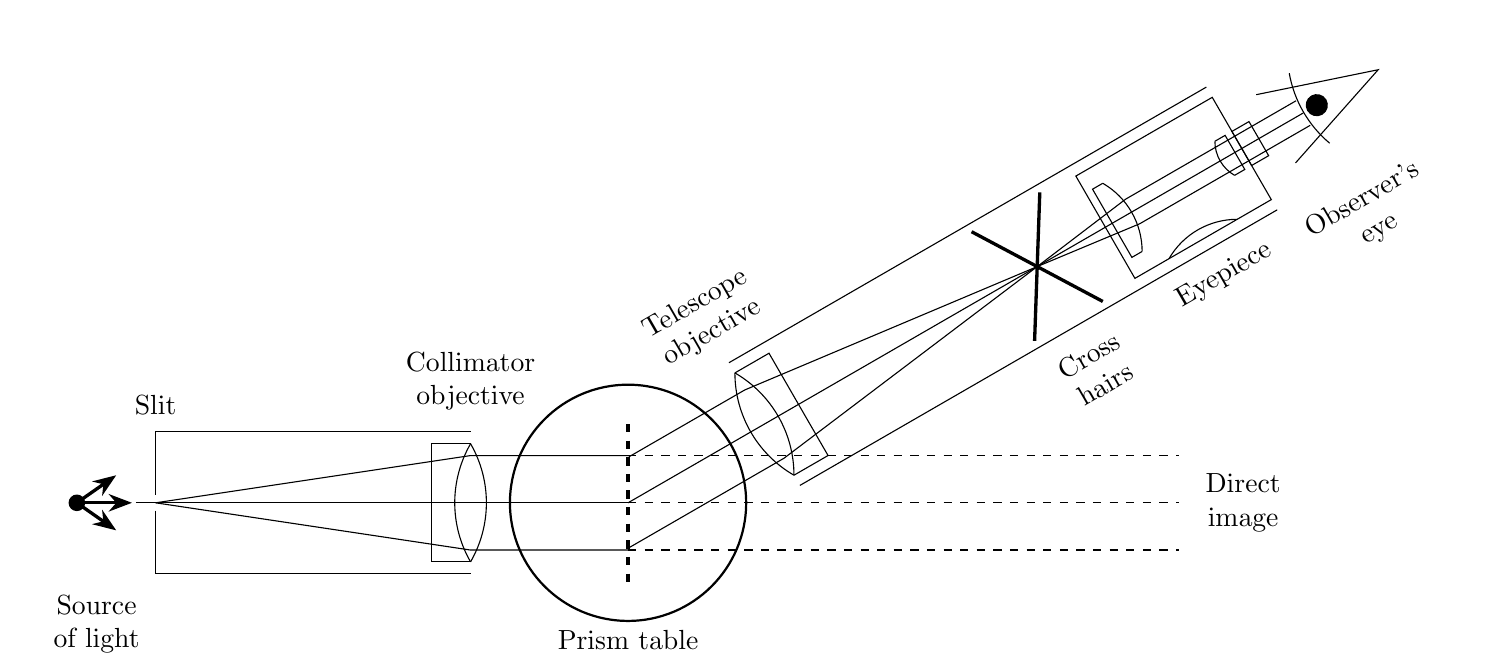
\begin{tikzpicture}
        \draw[thick] (6,0) circle (1.5);
        \draw (0,0.1) -- (0,0.9) -- (4,0.9);
        \draw (0,-0.1) -- (0,-0.9) -- (4,-0.9);
        \draw (4,0.75) arc[start angle=30, end angle=-30, radius=1.5];
        \draw (4,0.75) arc[start angle=150, end angle=210, radius=1.5];
        \draw (4,0.75) -- (3.5, 0.75) -- (3.5,-0.75) -- (4,-0.75);
        \draw [very thick, -Stealth] (-1,0) -- (-0.3,0);
        \draw [very thick, -Stealth] (-1,0) -- (-0.5,0.35);
        \draw [very thick, -Stealth] (-1,0) -- (-0.5,-0.35);
        % \draw [very thick, -Stealth] (-1,0) -- (-1,-0.5);
        % \draw [very thick, -Stealth] (-1,0) -- (-1,0.5);
        \fill[black] (-1,0) circle (3pt);
        \draw[very thick, dashed] (6,1) -- (6,-1);
        \draw (-0.25,0) -- (6,0);
        \draw (0,0) -- (4,0.6) -- (6,0.6);
        \draw (0,0) -- (4,-0.6) -- (6,-0.6);
        \node[below] at (-0.75,-1) {\begin{tabular}{c} Source \\ of light \end{tabular}};
        \node[above] at (0,1) {Slit};
        \node[above] at (4,1) {\begin{tabular}{c} Collimator \\ objective \end{tabular}}; 
        \node[below] at (6,-1.5) {Prism table};
        \begin{scope}[shift={(6,0)}]
          \begin{scope}[rotate=30, transform shape]
            \begin{scope}[shift={(-6,0)}]
            \draw (6,0) -- (15.9,0);
            \draw (6.3, 0.5) -- (8,0.5) -- (12,0) -- (13.4,-0.18) -- (15.9,-0.18);
            \draw (5.7, -0.5) -- (8,-0.5) -- (12,0) -- (13.4,0.18) -- (15.9,0.18);            
            \draw (8,0.75) arc[start angle=30, end angle=-30, radius=1.5];
            \draw (8,0.75) arc[start angle=150, end angle=210, radius=1.5];
            \draw (8,0.75) -- (8.5, 0.75) -- (8.5,-0.75) -- (8,-0.75);
            \draw (8,0.9) -- (15,0.9);
            \draw (8,-0.9) -- (15,-0.9);

        \draw (13.5,-0.75) arc[start angle=120, end angle=60, radius=1];
        \draw (14.75,0.25) arc[start angle=150, end angle=210, radius=0.5];
        \draw (14.75,0.25) -- (14.9,0.25) -- (14.9,-0.25) -- (14.75,-0.25);
        \draw (13.25,0.5) arc[start angle=30, end angle=-30, radius=1];
        \draw (13.25,0.5) -- (13.1,0.5) -- (13.1,-0.5) -- (13.25,-0.5);
            
            \draw (13,0.75) rectangle (15,-0.75);
            \draw[very thick] (11.5,0.8) -- (12.5,-0.8);
            \draw[very thick] (12.5,0.8) -- (11.5,-0.8);
            \node[above] at (8,1) {\begin{tabular}{c} Telescope \\ objective \end{tabular}};
            \node[below] at (12,-1) {\begin{tabular}{c} Cross \\ hairs \end{tabular}};
            \node[below] at (14,-1) {Eyepiece};
            \node[below] at (16,-1) {\begin{tabular}{c} Observer's \\ eye \end{tabular}};
            \draw (15,0.25) rectangle (15.25,-0.25);
            \fill[black] (16.1,0) circle (4pt);
            \draw (15.5,0.5) -- (17,0) -- (15.5,-0.5);
            \draw (16,-0.5) arc[start angle=200, end angle=160, radius=1.5];            
            \end{scope}
          \end{scope}
        \end{scope}  
        \draw [dashed] (6,0) -- (13,0);
        \draw [dashed] (6,0.6) -- (13,0.6);
        \draw [dashed] (6,-0.6) -- (13,-0.6);        
        \node[right] at (13,0) {\begin{tabular}{c} Direct \\ image \end{tabular}};
    \end{tikzpicture}
    \caption{An optical arrangement of a spectroscope set to observe the spectrum of a light source in some non-zero diffraction order.}
    \label{Spectroscope}
\end{figure}

Regardless of the type of dispersive element used, the most important characteristics of a spectrometer are its \textit{resolving power}, \textit{dispersion}, and \textit{free spectral range}. 

The resolving power characterizes the ability of an instrument to separate (i.e. resolve) two very close spectral lines with wavelengths $\lambda$ and $\lambda + \delta \lambda$ as distinct, separate lines, and is given by $R = \lambda/\delta \lambda$. A certain criterion needs to be established to define what one means by resolving the two spectral lines. According to the \textit{Rayleigh criterion}, two spectral lines of equal intensity are just resolved if the first diffraction minimum of one falls onto the maximum of the other at some angle $\theta$.%for chromatic resolving power 

One can show that the resolving power of a grating is given by the product of the diffraction order, $m$, and the total number $N$ of working (illuminated) apertures in the grating: $R = m N$. An equivalent way of expressing this is $R = (d \sin \theta/\lambda) (w/a) = w \sin \theta /\lambda$, where $d$ is the grating spacing and $w$ is the full width of the grating. Hence the resolving power is equal to the number of wavelengths in the path difference of waves arriving from opposite edges of the grating. Therefore, for a given wavelength and angle, the power to resolve spectral lines is \textit{independent} of the grating spacing! To increase the resolving power, one needs to make the grating larger or to increase the angle of diffraction (or both).

The dispersion of a spectrometer is a measure of the deviation of light depending on its wavelength. The angular dispersion $\text{d}\theta/\text{d}\lambda$ measures the variation with wavelength of the deviation angle, and for a grating spectrometer is given by $\text{d}\theta/\text{d}\lambda = m/(d \cos \theta)$, where $d$ is the grating spacing and $m$ is the diffraction order.

The free spectral range is the spectrum interval $\Delta \lambda$ that can be observed without overlap from other wavelengths in the incident radiation. For a diffraction grating the free spectral range is $\Delta \lambda = \lambda/m$, i.e. is determined only by the diffraction order $m$ for the given wavelength. The larger the order $m$, the narrower the free spectral range.

\begin{figure}[ht!]
    \centering
    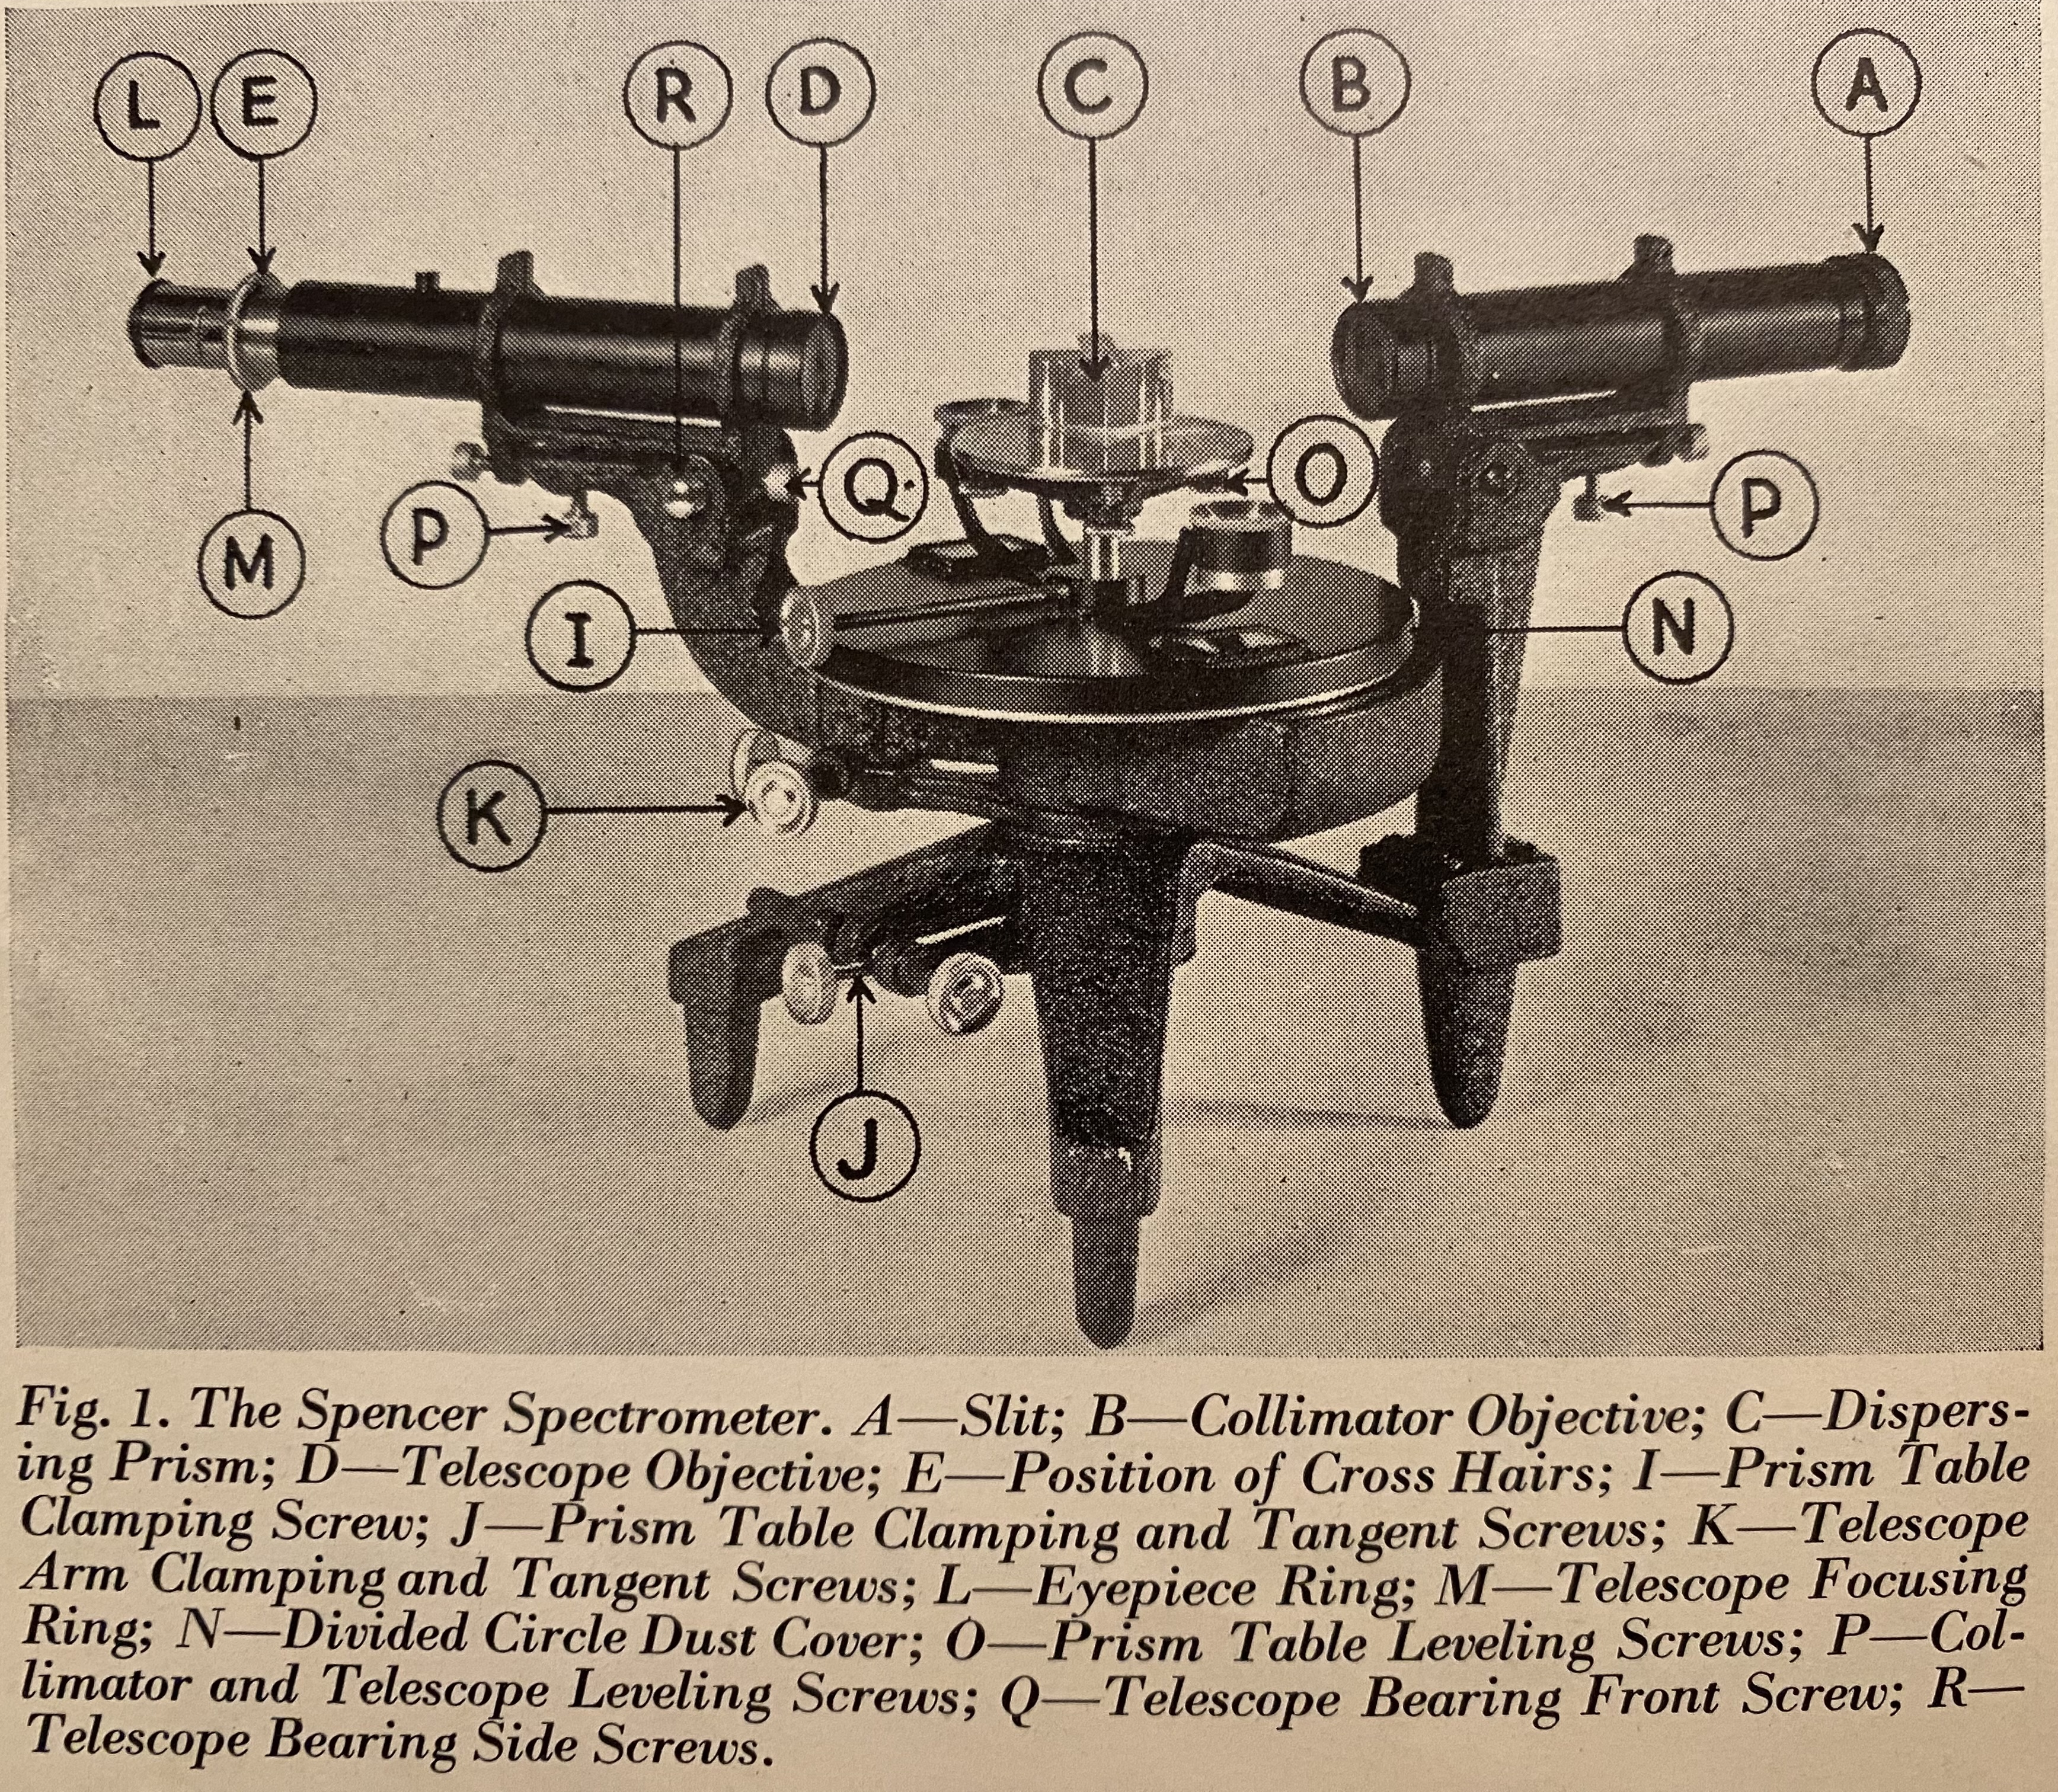
\includegraphics[width=0.85\linewidth]{Fig-1-The-Spencer-Spectrometer.jpg}
    \caption{The Spencer spectrometer (adapted from the manual by Roger S. Astey).}
    \label{Spencer Spectrometer}
\end{figure}

\section{Optical Alignment of the Spencer Spectrometer}

Prior to making precise measurements, the spectrometer needs to be carefully adjusted. The procedure generally consists of the following steps, usually done in this order: 1)~focusing the telescope for parallel rays; 2)~focusing the collimator for parallel rays; 3)~setting the telescope and collimator axes perpendicular to the principal mechanical axis of the instrument; 4)~adjusting the dispersive element (a prism or diffraction grating) used in measurements.

\subsection{Focusing the Telescope}
One begins by adjusting the telescope with the goal of positioning the cross hairs at the common focal plane of the telescope objective and the eyepiece.

\begin{enumerate}
    \item To focus the eyepiece on the cross hairs, carefully pull the eyepiece by the ring $L$ \textit{almost} out of the telescope tube and then insert it slowly until a sharp image of the cross hairs is seen with a naked eye.\footnote{In using the spectrometer and other optical instruments, it is unnecessary to wear prescription glasses which correct near- or far-sightedness, since the change in focus of the eyepiece accomplishes the same purpose (the eyepiece, however, will \textit{not} correct for astigmatism). In addition, various protective coatings on lenses designed to block harmful UV radiation may severely limit the transmission of some spectral lines closer to the violet end of the visible spectrum.} To avoid eye fatigue, position the eyepiece inside the tube as far out as possible while still allowing for a sharp image of the cross hairs to be seen (the goal is to push the virtual image of the cross hairs to infinity).
\end{enumerate}

The eyepiece adjustment may be changed, if necessary, at any point during the experiment to suit another observer’s eye, or if the eyepiece is accidentally disturbed.

\begin{figure}[ht!]
    \centering
    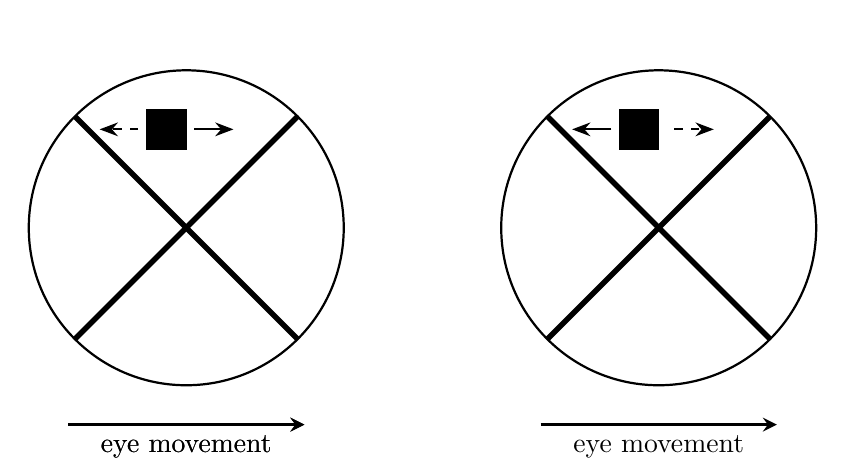
\begin{tikzpicture}
        \draw[thick] (0,0) circle (2);
        \draw[line width=2pt] (-1.41,1.41) -- (1.41,-1.41);
        \draw[line width=2pt] (-1.41,-1.41) -- (1.41,1.41);
        \draw[thick] (6,0) circle (2);
        \draw[line width=2pt] (4.59,1.41) -- (7.41,-1.41);
        \draw[line width=2pt] (4.59,-1.41) -- (7.41,1.41);
        \filldraw[black] (-0.5,1) rectangle (0,1.5);
        \draw[thick, -Stealth] (0.1,1.25) -- (0.6,1.25);
        \draw[thick, dashed, -Stealth] (-0.4,1.25) -- (-1.1,1.25);  
        \filldraw[black] (5.5,1) rectangle (6,1.5);
        \draw[thick, -Stealth] (5.4, 1.25) -- (4.9,1.25); 
        \draw[thick, dashed, -Stealth] (6.2, 1.25) -- (6.7,1.25);
        \draw[very thick, -stealth] (-1.5,-2.5) -- (1.5,-2.5) node[midway, below] {eye movement};
        \draw[very thick, dashed, -stealth] (1.5,-3.25) -- (-1.5,-3.25);      
        \draw[very thick, -stealth] (-1.5,-2.5) -- (1.5,-2.5) node[midway, below] {eye movement};
        \draw[very thick, -stealth] (4.5,-2.5) -- (7.5,-2.5) node[midway, below] {eye movement};
        \draw[very thick, dashed, -stealth] (7.5,-3.25) -- (4.5,-3.25);       
    \end{tikzpicture}
    \caption{Movement of the image of a distant object  as seen in the telescope as the observer's eye moves laterally in front of the eyepiece. \textbf{Left:} the cross hairs are \textbf{closer} to the objective than the focal point. \textbf{Right:} the cross hairs are \textbf{farther away} from the objective than the focal point. This parallax is eliminated when the cross hairs are exactly at the focal point of the objective.}
    \label{Eye movement}
\end{figure}

The simplest way of adjusting the focus of the objective lens is to point the telescope tube towards a very distant object, preferably through an open window or door, and eliminate parallax between the virtual image of the object and the cross hairs. This is a good preliminary step even if the most ``distant" object accessible to you is just a few tens of feet away across the room, especially when the objective lens is far out of alignment.

\begin{enumerate}[resume]
\item To focus the objective lens point the telescope towards the most distant unobstructed object you can find in the horizontal plane. Adjust the knurled ring~$M$ to obtain a sharp image of the distant object and then eliminate parallax between the image and the cross hairs: if the cross hairs are in the focal plane of the objective lens, as you move your eye slightly laterally from side to the side, the cross hairs are fixed on the distant object. If they are inside/outside the focal plane, the image of the distant object moves in the same/opposite direction to the eye movement (see Figure \ref{Eye movement}). Slowly adjust the knurled ring $M$ until the cross hairs are \textbf{fixed} on the distant object.
\end{enumerate}

\subsection{The Autocollimation Method}

The Gauss eyepiece used in the Spencer spectrometer allows for a much more precise focusing of the objective lens using the autocollimation method applicable in the dark room environment. The cross hairs are illuminated through the side window in the eyepiece by means of an auxiliary source of light directed towards a thin transparent piece of glass making an angle of 45 degrees with the optical axis of the telescope. Upon emerging from the telescope objective, the light beam is allowed to reflect from a planar surface, such as the surface of a mirror or the polished face of a prism (see Figure \ref{Autocollimation Method}). Elimination of parallax between the two images of cross hairs seen in the telescope puts the objective lens in focus.

\begin{figure}[ht!]
    \centering
    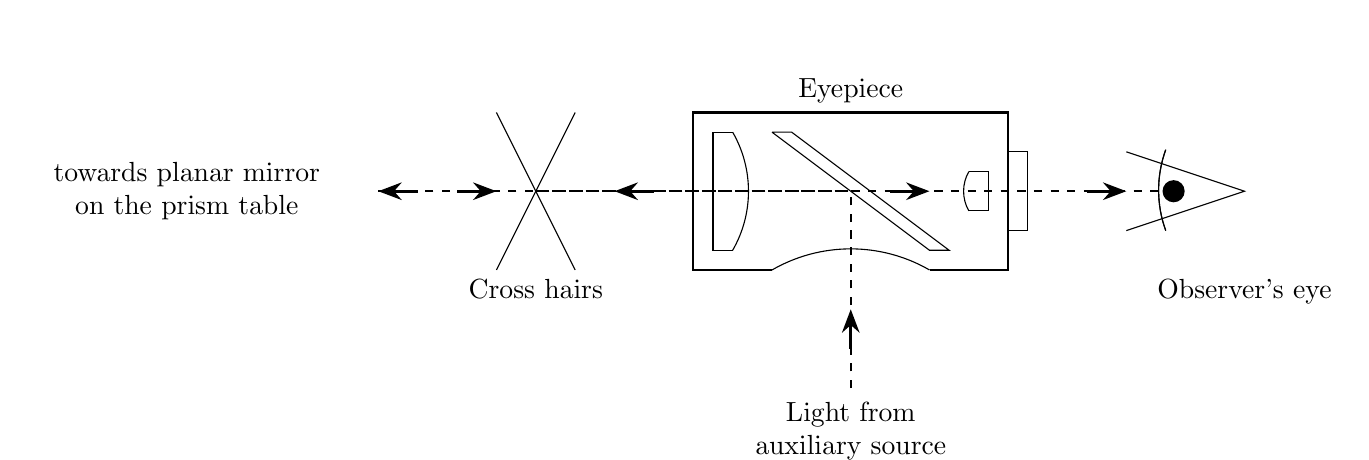
\begin{tikzpicture}
        \draw[thick] (7,-1) -- (6,-1) -- (6,1) -- (10,1) -- (10,-1) -- (9,-1);
        \draw (7,-1) arc[start angle=120, end angle=60, radius=2];
        \draw (12,-0.5) arc[start angle=200, end angle=160, radius=1.5];
        \draw(6.5,-0.75) -- (6.25,-0.75) -- (6.25,0.75) -- (6.5,0.75);
        \draw (9.5,0.25) arc[start angle=150, end angle=210, radius=0.5];
        \draw (9.5,0.25) -- (9.75,0.25) -- (9.75,-0.25) -- (9.5,-0.25);
        \draw (10,0.5) rectangle (10.25,-0.5); 
        \draw (6.5,0.75) arc[start angle=30, end angle=-30, radius=1.5];
        \fill[black] (12.1,0) circle (4pt);
        \draw (11.5,0.5) -- (13,0) -- (11.5,-0.5);
        \draw (12,-0.5) arc[start angle=200, end angle=160, radius=1.5];
        \draw (7,0.75) -- (7.25,0.75) -- (9.25,-0.75) -- (9,-0.75) -- (7,0.75);

        \draw[dashed, thick] (8, -2.5) -- (8,0) -- (2,0);
        \draw[dashed, thick] (4,0) -- (12,0);
        \draw[very thick, -Stealth] (11,0) -- (11.5,0);
        \draw[very thick, -Stealth] (8,-2)--(8,-1.5);
        \draw[very thick, -Stealth] (5.5,0)--(5,0);
        \draw[very thick, -Stealth] (8.5,0)--(9,0);
        \draw[very thick, -Stealth] (3,0)--(3.5,0);
        \draw[very thick, -Stealth] (2.5,0)--(2,0);

        \node[right,xshift=-70pt] (0,0) {\begin{tabular}{c} towards planar mirror \\ on the prism table \end{tabular}};
        \draw (3.5,1) -- (4.5,-1); \draw (4.5,1) -- (3.5,-1);
        \node[below] at (4,-1) {Cross hairs};
        \node[below] at (8,-2.5) {\begin{tabular}{c} Light from \\ auxiliary source \end{tabular}};
        \node[below] at (13,-1) {Observer's eye};
        \node[above] at (8,1) {Eyepiece};
    \end{tikzpicture}
    \caption{The passage of light in the autocollimation method. }
    \label{Autocollimation Method}
\end{figure}

\textbf{The aluminum mirror used in this experiment is extremely delicate and has a very thin (hundreds of nanometers) protective silicon dioxide coating deposited on top of an even thinner aluminum reflective coating. Never touch the surface of the mirror (even with gloves) or attempt to clean it in any way. Do NOT breathe on or blow air toward the mirror. Keep the protective cover on when not in use. Mount and unmount the mirror on the prism table with the protective cover~ON.}
\begin{enumerate}
    \item Approximately level the telescope tube using the leveling screw $P$, the associated radial clamp, and a spirit level. Level the prism table using the leveling screws $O$.
    \item Open the window $G$ in the Gauss eyepiece by rotating the ring $L$ and illuminate the cross hairs with an auxiliary source of light. Adjust the ring $L$ and the auxiliary source to achieve uniform and bright field of view (the two little circles you see are images of the frosted glass illuminated by a white LED inside the auxiliary source).
    \item Secure onto the prism table a highly reflective mirror in its mount. Carefully position the mirror's mount with respect to three leveling screws $O$ to allow for a controlled tilt of the mirror's surface (the plane of the mirror should be perpendicular to the line connecting two of the three leveling screws, see Figure \ref{Mirror Placement}).
\begin{figure}[ht!]
    \centering
    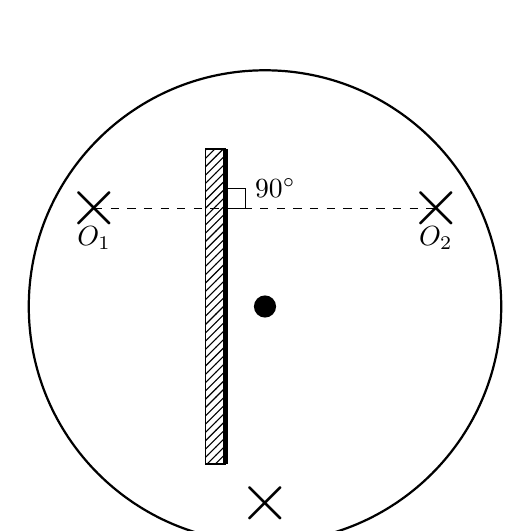
\begin{tikzpicture}
        \draw[thick] (0,0) circle (3);
        \fill[black] (0,0) circle (4pt);
        \draw[pattern=north east lines] (-0.75,2) rectangle (-0.5,-2);
        \draw[ultra thick] (-0.5,2) -- (-0.5,-2);
        \node at (0,-2.5) {\Huge $\times$};
        \node at (-2.17,1.25) {\Huge $\times$};
        \node[below,yshift=-3pt] at (-2.17,1.25) {$O_1$};
        \node[below,yshift=-3pt] at (2.17,1.25) {$O_2$};
        \node at (2.17,1.25) {\Huge $\times$};
        \draw[dashed] (-2.17,1.25) -- (2.17,1.25);
        \draw (-0.5, 1.25) rectangle (-0.25,1.5) node[above,right] {$90^{\circ}$};
    \end{tikzpicture}
    \caption{The correct placement of the mirror on the prism table in relation to the three leveling screws at the vertices of an equilateral triangle. $O_1$ and $O_2$ allow for the mirror's~tilt.}
    \label{Mirror Placement}
\end{figure}    
    \item Using the clamping screw $I$ set the height of the prism table such that most of the light beam emerging from the illuminated objective lens will fall onto the mirror's surface.
    \item Carefully open the protective cover on the mirror and make the telescope tube approximately normal to the mirror's surface. Gently rotate the prism table by the dust cover $N$ and use an index card to locate a reflected circle of light in the plane of the objective lens (see Figure \ref{Reflected circle of light}).
    
\begin{figure}[ht!]
    \centering
    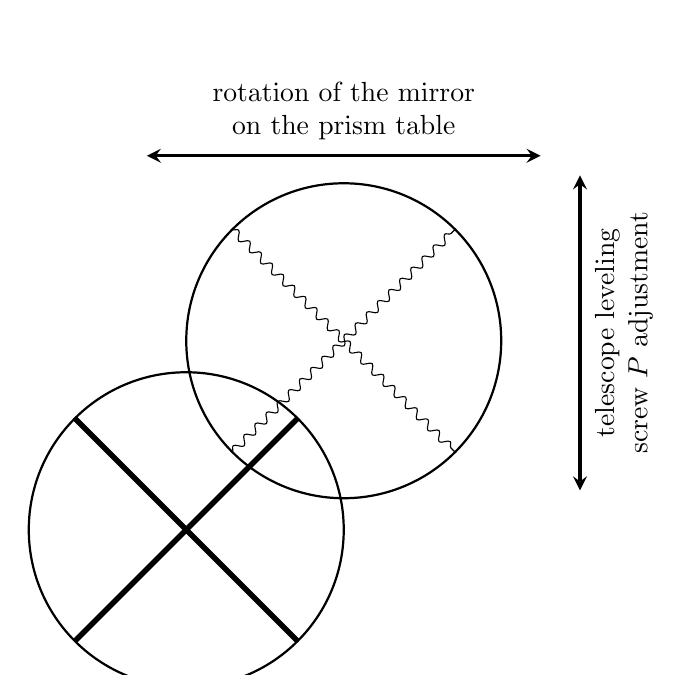
\begin{tikzpicture}
        \def\r{2} % radius of circle
        \def\a{45} % reticle angle
        \coordinate (A) at ({-\r*cos(\a)},{\r*sin(\a)},0);
        \coordinate (B) at ({\r*cos(\a)},{-\r*sin(\a)},0);
        \coordinate (C) at ({-\r*cos(\a)},{-\r*sin(\a)},0);
        \coordinate (D) at ({\r*cos(\a)},{\r*sin(\a)},0);
        \coordinate (O) at ({\r},{1.2*\r});
        \coordinate (E) at ({\r-\r*cos(\a)},{1.2*\r+\r*sin(\a)},0);
        \coordinate (F) at ({\r+\r*cos(\a)},{1.2*\r-\r*sin(\a)},0);
        \coordinate (G) at ({\r-\r*cos(\a)},{1.2*\r-\r*sin(\a)},0);
        \coordinate (H) at ({\r+\r*cos(\a)},{1.2*\r+\r*sin(\a)},0);            
        \draw[thick] (0,0) circle (\r);
        \draw[line width=2pt] (A) -- (B);
        \draw[line width=2pt] (C) -- (D);
        \draw[thick] (O) circle (\r);
        \draw[decorate, decoration={snake, amplitude=0.5mm, segment length=2mm}] (E) -- (F);
        \draw[decorate, decoration={snake, amplitude=0.5mm, segment length=2mm}] (G) -- (H);   
        \draw[very thick, stealth-stealth] (-0.5,4.75) -- (4.5,4.75) node[midway, above] {\begin{tabular}{c} rotation of the mirror \\ on the prism table \end{tabular}};
        \draw[very thick, stealth-stealth] (5,0.5) -- (5,4.5) node[midway, below, rotate=90] {\begin{tabular}{c} telescope leveling \\ screw $P$ adjustment \end{tabular}};
    \end{tikzpicture}
    \caption{The direct and reflected images of cross hairs in the autocollimation method. }
    \label{Reflected circle of light}
\end{figure} 

    \item Use the leveling screws $O_1$ and $O_2$ to tilt the mirror and rotate the prism table by the dust cover $N$ to make the reflected circle of light partially intersect the direct image as shown in Figure \ref{Reflected circle of light}. Be careful not to completely unfasten any leveling screws $O$ nor to over-screw them so they protrude from the prism table surface! 
    \item Look into the telescope tube and observe the reflected circle of light with the second set of fuzzy cross hairs. Put in good focus this reflected image of the cross hairs by slowly adjusting the knurled ring $M$ (as you can see, the preliminary focus using a ``distant" object was only approximate). 
    \item Secure the telescope and prism table by using the radial clamping screws $K$ and~$J$, respectively. Use the fine adjustment tangential screw $J$ and the telescope leveling screws~$P$ to bring the reflected and direct images of the cross hairs almost into coincidence.
    \item Eliminate parallax between the direct and reflected images of the cross hairs by slowly adjusting the knurled ring $M$.
\end{enumerate}
\textbf{After the telescope objective is adjusted, the knurled ring $M$ should not be disturbed for the duration of the experiment.}

\subsection{Focusing the Collimator}
The next step is to set the collimator slit exactly in the focal plane of the collimator objective. This can be achieved by using the well adjusted telescope. For this lab  \textbf{the collimator has been focused ahead of time}. You can use the clamping ring on the draw tube to position the collimator slit $A$ vertically or horizontally by aligning the corresponding V-shaped tongue and grooves on the collimator tube (push the tongue all the way into the groove).
\begin{enumerate}
    \item Close the cap on the mirror mount and carefully remove the mirror from the prism table. Align the telescope with the collimator.
    \item Using one of the gas discharge tubes with a noble gas in it, illuminate evenly the vertical collimator slit $A$ which should be moderately open. Make sure the capillary tube is centered on the slit and the entire length of the slit is well illuminated. To better see jaws of the collimator slit, illuminate the objective of the collimator with a flash light. Be sure not to touch the slit itself or the gas discharge lamp.
    \item Check that there is no parallax between the intersection of the cross hairs and the image of the narrow vertical slit. If successful, continue with section 3.4 below.
    \item If there is parallax, most likely, the telescope was not adjusted properly. Use the knurled ring $M$ to make small adjustments and eliminate parallax. \textbf{Ask the TA} to check your telescope focus. If necessary, the TA will complete the last step.
    \item \textbf{TA ONLY IF NECESSARY:} Align the corresponding V-shaped tongue and grooves on the collimator tube (push the tongue all the way into the groove) to make the slit vertical. If with a well-adjusted telescope the collimator slit is not in focus, unclamp the collimator ring using a flat-head screwdriver and slide the draw tube of the collimator in and out to approximately focus on the image of the  slit seen in the telescope. Use a flashlight to better see the jaws of the slit. Eliminate parallax between the cross hairs and the slit image. Re-clamp the ring using the flat-head screwdriver and check for parallax again.
\end{enumerate}

\subsection{Setting the Telescope and Collimator Axes Perpendicular to the Bearing Axis}
For precise spectroscopic measurements it is important to set the intersection of the cross hairs in the geometrical plane normal to the principal mechanical axis of rotation (the bearing axis of the instrument around which both the telescope and the collimator tubes rotate).
\begin{enumerate}
    \item Carefully rotate the draw tube holding the metal clamping ring (\textbf{not} the plastic slit adjustment ring!) to position the collimator slit horizontally (align the matching V-shaped tongue and groove). Illuminate evenly the collimator slit $A$ with light from one of the gas discharge tubes with a noble gas in it. The slit should be almost closed. Make sure the capillary tube is centered on the slit and the entire length of the slit is well illuminated. Bring the horizontal slit image into coincidence with the intersection of the cross hairs by adjusting the leveling screws $P$ on \textit{either} the telescope \textit{or} the collimator. \textbf{Tighten the corresponding radial screw}. Double check the coincidence.
\end{enumerate}

The telescope and collimator axes are now parallel. They have also been made to intersect the mechanical axis by adjusting screws $Q$ and $R$ (do NOT disturb these!), so the axes are also \textit{nearly} coincident. However, the telescope and collimator axes are NOT necessarily perpendicular to the bearing axis of the instrument (see Figure \ref{Bearing axis}). To make them perpendicular, first use the mirror to set the reflecting surface normal to the bearing axis.

\begin{figure}[ht!]
    \centering
    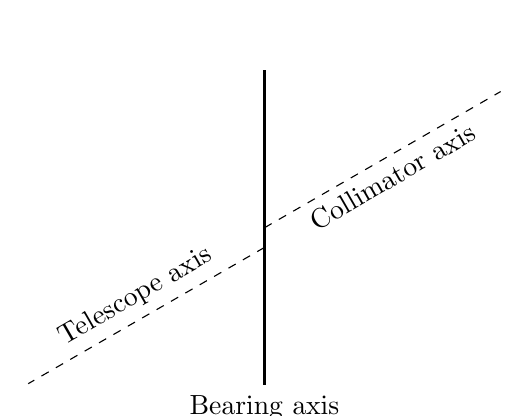
\begin{tikzpicture}
        \draw[thick] (0,4) -- (0,0) node[below] {Bearing axis};
        \draw[dashed] (0,2) -- (3,3.73) node[midway, below, sloped] {Collimator axis};
        \draw[dashed] (0,1.75) -- (-3,0.02) node[midway, above, sloped] {Telescope axis};        
    \end{tikzpicture}
    \caption{Exaggerated view of the telescope and collimator axes not perpendicular to the bearing axis of the instrument, each making identical angles with the latter.}
    \label{Bearing axis}
\end{figure}

\begin{enumerate}[resume]
    \item Rotate the telescope tube until it is approximately normal to the collimator tube and set the mirror on the prism table to reflect light from the collimator into the telescope as in Figure \ref{Telescope normal to collimator}.

\begin{figure}[ht!]
    \centering
    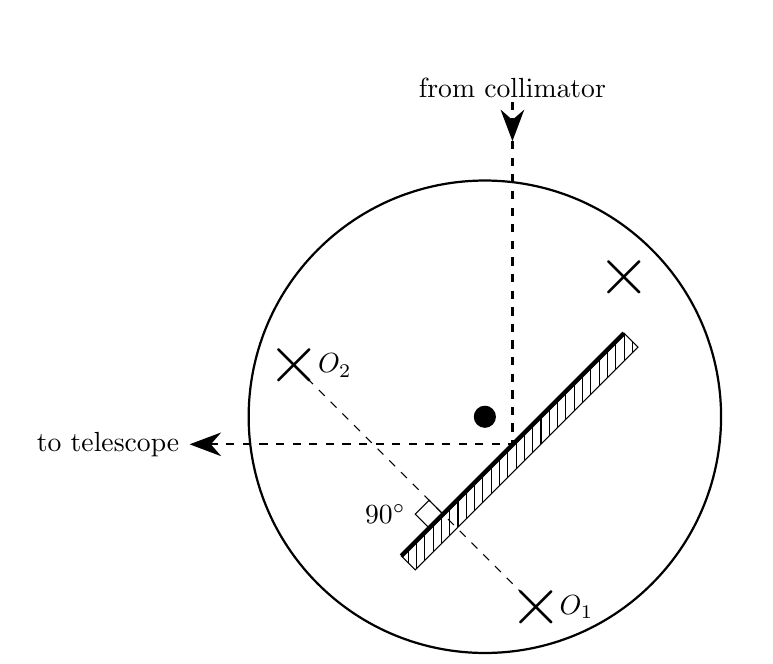
\begin{tikzpicture}
        \begin{scope}[rotate=135]
        \draw[thick] (0,0) circle (3);
        \fill[black] (0,0) circle (4pt);
        \draw[pattern=vertical lines] (-0.75,2) rectangle (-0.5,-2);
        \draw[ultra thick] (-0.5,2) -- (-0.5,-2);
        \node at (0,-2.5) {\Huge $\times$};
        \node at (-2.17,1.25) {\Huge $\times$};
        \node at (2.17,1.25) {\Huge $\times$};
        \node[right, xshift=5pt] at (-2.17,1.25) {$O_1$};
        \node[right, xshift=5pt] at (2.17,1.25) {$O_2$};        
        \draw[dashed] (-2.17,1.25) -- (2.17,1.25);
        \draw (-0.5, 1.25) rectangle (-0.25,1.5) node[above,left] {$90^{\circ}$};
        \end{scope}
        \draw[thick, dashed, -{Stealth[length=4mm,width=3mm]}] (0.35,4) -- (0.35,3.5);
        \draw[thick, dashed, -{Stealth[length=4mm,width=3mm]}] (0.35,3.5) node[above, yshift=12pt] {from collimator} -- (0.35,-0.35) -- (-3.75,-0.35) node[left] {to telescope};
    \end{tikzpicture}
    \caption{The mirror surface is made perpendicular to the bearing axis of the spectrometer by setting it to reflect light from the collimator into the telescope and adjusting its tilt until the horizontal slit image coincide with the intersection of the cross hairs.}
    \label{Telescope normal to collimator}
\end{figure}
    
    \item Adjust the tilt of the mirror using leveling screws $O_1$ \textbf{and} $O_2$ and carefully rotate the prism table to make the slit image and the intersection of cross hairs coincide.
\end{enumerate}
Now the surface of the mirror is perpendicular to the bearing axis of the instrument, and the telescope and collimator axes each make an identical angle with the bearing axis (illustrate this with a diagram). Use autocollimation to make the telescope axis normal to the mirror.
\begin{enumerate}[resume]
    \item Rotate the prism table to set the mirror on it approximately normal to the telescope axis, and then adjust the telescope leveling screw $P$ to bring the direct and reflected images of the cross hairs into coincidence. Clamp the telescope tube using the radial screw near P. Do \textbf{NOT} tilt the already adjusted mirror!
\end{enumerate}
The telescope axis is now normal to the bearing axis. Adjust the collimator  accordingly.
\begin{enumerate}[resume]
    \item Close the cap on the mirror mount, remove the mirror from the prism table and bring the telescope in alignment with the collimator. Adjust the collimator leveling screw P until the slit image and the intersection of cross hairs coincide.  The collimator axis is now normal to the bearing~axis.
\end{enumerate}

 \begin{enumerate}[resume]
    \item Turn the collimator slit into the vertical position by aligning the V-shaped tongue on the ring clamp with the corresponding  groove on the tube. Check again for parallax and adjust if necessary. Close the window G, otherwise you will see two images of the slit by allowing stray light into the telescope.
\end{enumerate}

\subsection{Adjusting the Dispersive Element}
A diffraction grating used in spectroscopic measurements needs to be carefully adjusted. Its grooves are made parallel to the (now vertical) collimator slit and then the grating is adjusted for normal incidence in relation to the collimator.  Gratings used in this experiment are high quality replicas of original (ruled) gratings produced by Paton Hawksley. A thin layer of resin cast from the original is adhered between two protective glass plates bound together at edges.
\begin{enumerate}
    \item Attach the diffraction grating mount to the prism table using a screw and a hex key. Holding the diffraction grating \textbf{by its edges}, carefully set the slide inside the mount and center it. Mount the grating on the prism table using a hex key and a screw. The grating surface should \textbf{bisect} the distance between two of the leveling screws, $O_1$ and $O_2$, which are used to tilt the grating surface. Lower the prism table to adjust its height so that the entire collimated beam passes through the grating area of the~slide. 
    \item To ease future readings of the vernier scales through glass windows in the dust cover $N$, rotate the cover and unclamped prism table to align the two windows and the grating surface set approximately normal to the collimator axis. Use the clamping screw $I$ to clamp the prism table.
    \item Set the telescope approximately normal to the collimator and rotate the prism table so that the protective glass cover of the grating reflects light from the collimator into the telescope.
    \item Adjust the tilt of the diffraction grating using the leveling screws $O_1$ and $O_2$ \textbf{equally} to make the intersection of the cross hairs level with the image of the horizontal slit (tilt the grating surface \textit{half} the needed angle with screw $O_1$ and then complete the centering with screw $O_2$).
\end{enumerate}
The plane of the grating is now vertical, but the grooves may NOT be vertical.
\begin{enumerate}[resume]
    \item Rotate the slit into the vertical position and align the telescope with the collimator.
    \item Rotate the prism table to position the grating approximately perpendicular to the collimator axis. 
    \item Locate the central image of the slit (the zeroth diffraction order). Rotate the telescope to observe the first and second order spectra on both sides from the central image. You may see a skewed image of spectral lines as in Figure \ref{Skewed image of spectral lines}.
\end{enumerate}

\begin{figure}[ht!]
    \centering
    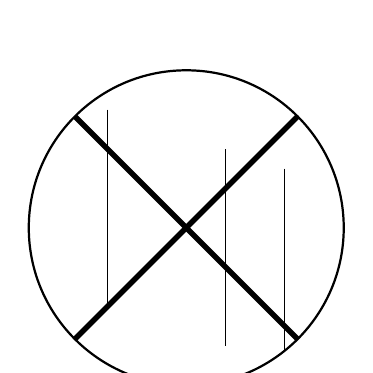
\begin{tikzpicture}
        \draw[thick] (0,0) circle (2);
        \draw[line width=2pt] (-1.41,1.41) -- (1.41,-1.41);
        \draw[line width=2pt] (-1.41,-1.41) -- (1.41,1.41);
        \draw (-1,1.5) -- (-1,-1);
        \draw (0.5,1) -- (0.5,-1.5);
        \draw (1.25,0.75) -- (1.25,-1.55);
    \end{tikzpicture}
    \caption{Skewed image of spectral lines in relation to the cross hairs as a result of the grooves of the diffraction grating not being parallel to the vertical collimator slit.}
    \label{Skewed image of spectral lines}
\end{figure}

\begin{enumerate}[resume]
    \item Adjust the leveling screw that leaves the grating surface parallel to itself to make the grooves vertical (the intersection of the cross hairs should fall onto the center of the spectral lines at all orders observed). If the travel of this leveling screw is not enough to , rotate the grating in its mount by pressing down and holding one of its top corners and moving up the other top corner (see Figure \ref{Grating rotation}).
\end{enumerate}

\begin{figure}[ht!]
    \centering
    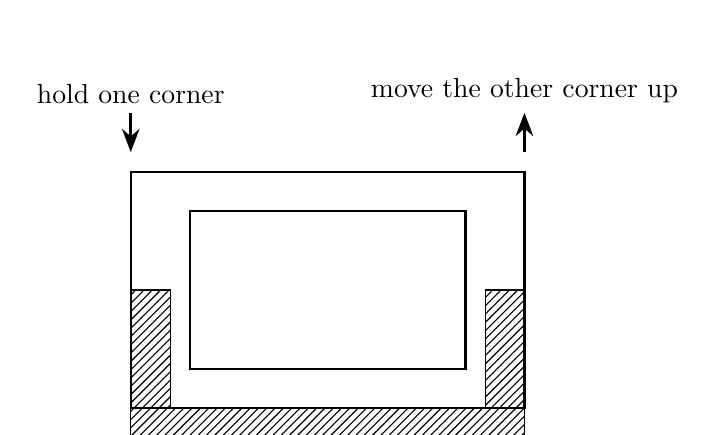
\begin{tikzpicture}
        \draw[pattern=north east lines] (0,0) rectangle (5,0.5);
        \draw[thick] (0,0.5) rectangle (5, 3.5);
        \draw[thick] (0.75,1) rectangle (4.25,3);        
        \draw[pattern=north east lines] (0,0.5) rectangle (0.5,2);
        \draw[pattern=north east lines] (4.5,0.5) rectangle (5,2);
        \draw[very thick, -Stealth] (0, 4.25) -- (0, 3.75);
        \node[above] at (0,4.25) {hold one corner};        
        \draw[very thick, -Stealth] (5, 3.75) -- (5, 4.25);
\node[above] at (5,4.25) {move the other corner up};        
    \end{tikzpicture}
    \caption{Demonstration of the diffraction grating  rotation in its mount.}
    \label{Grating rotation}
\end{figure}

The grooves of the grating are now parallel to the collimator slit. To adjust the grating for normal incidence in relation to the collimator, one can set its surface perpendicular to the collimator axis (i.e. make the angle of incidence zero)
\begin{enumerate}[resume]
    \item First align the intersection of the cross hairs on the central image of the slit (zeroth diffraction order).
    \item Use the autcollimation method to make the protective glass surface of the grating perpendicular to the telescope axis.
\end{enumerate}
To independently check this alignment, verify the equality of the diffracted angles of the same order on both sides of the central image.

\newpage
\section{Measurements}
The goal of this experiment is an accurate determination of the energy of the light quanta emitted by the Hydrogen atom in its transitions to the second energy state. To achieve a better accuracy in determining the corresponding wavelengths, the diffraction grating spacing is first accurately determined using strong lines in the spectrum of neutral helium as standards.

\subsection{Determination of the Grating Spacing}
After the spectrometer is adjusted using the optical alignment procedure described in the previous section, one begins with an accurate determination of the diffraction grating spacing. The nominal value of the spacing provided by the manufacturer (600 lines/mm) is only \textit{approximate}, as no two diffraction gratings are exactly alike. Furthermore, the grating spacing varies depending on the region of the grating illuminated by the collimator. This is a consequence of the fabrication process, in which a replica of the grating is made by peeling a resin layer from an original ruled grating, a step that inevitably introduces various deformations contributing to variations in the grating spacing.
\begin{enumerate}
    \item Select three to four prominent and visually identifiable lines in the emission spectrum of helium given in the table below.
    \begin{table}[ht!]
    \centering
    \begin{tabular}{|c|c|c|}
    \hline
    Wavelength in air, \AA & Color & Relative intensity \\
    \hline
    % Hg & 4046.563  & violet & 2 & 400 P\\
    % Hg & 4347.494 & violet & --- & 100 \\
    % Hg & 4358.343 & violet(blue) & 8 & 1000 P\\
    4471.4 & violet & 200/25\\
    4713.1 & blue & 30/40\\
    % Ne & 4849 & blue-green & 8 & --- \\
    4921.9 & blue-green & 20\\
    5015.7 & green &  100\\
    5047.7 & green & 10 \\
    % Ne & 5037.7512 & green & 5 & 50\\
    % Ne & 5330.7775 & green & 8 & 60 \\
    % Ne & 5400.5618 & green & 6 & 200 P\\
    % Hg & 5460.742 & green & 10 & 500 P\\
    % Ne & 5764.418 & bright-green & 4 & 70\\
    % Hg & 5769.598 & yellow & 8 & 50 \\
    % Hg & 5790.659 & yellow & 10 & 60\\
    % Ne & 5852.4879 & yellow & 20 & 200 P\\
    5875.6 & yellow & 500/250/120 P\\
    % Ne & 5881.8952 & orange? & --- & 100\\
    % Ne & 5945 & orange & 5 & 50\\
    % Ne & 6029.9969 & red-orange & --- & 100 P\\
    % Ne & 6074.3377 & red-orange & --- & 100 P\\
    % Ne & 6143.0626 & red-orange & 10 & 100 P\\
    % Ne & 6163.5939 & red & --- & 100 P\\
    % Ne & 6217.2812 & red & --- & 100 P\\
    % Ne & 6266.4950 & red & --- & 100 P\\
    % Ne & 6382.9917 & red & --- & 100 P\\
    % Ne & 6402.248 & bright red & 10 & 200 P\\
    % Ne & 6506.5281 & red & --- & 150 P\\
    % Ne & 6598.9529 & red & --- & 100 P\\
    6678.1 & bright red & 200 P\\
    % Ne & 6929.4673 & very bright  red & --- & 1000 P\\
    % Ne & 7032.4131 & very bright red & --- & 800 P\\
    7065.2 & red & 100/60/20 P\\
    % Hg & 7081.90 & red & --- & 25\\
    \hline       
    \end{tabular}
        \caption{Strong emission lines in the spectrum of helium. Relative intensities are given using the NIST \href{https://physics.nist.gov/PhysRefData/Handbook/Tables/heliumtable2.htm}{data}. If a line has a doublet or triplet structure, the wavelength of the strongest line is shown. The wavelengths are given in air with a refractive index of 1.00029 in the visible region.}\label{strong_helium_lines}
    \end{table}  
    \item The diffraction grating should be already adjusted in accordance with section~1.4 above, including the adjustment for normal incidence in relation to the collimator.
    \item \textbf{Without disturbing this adjustment}, clamp the prism table using the screw~$J$ and align the telescope axis with the collimator by using the clamping and tangent screws~$K$. Align the intersection of the cross hairs with the center of the narrow collimator slit.
    \item For correct alignment, the fuzzy reflected images of the cross hairs obtained by illuminating the glass covers of the grating with auxiliary light via the open window $G$ in the eyepiece must be centered on the direct image of the cross hairs, which is simultaneously centered on the image of the narrow collimator slit. Close the window $G$ by rotating the ring $L$ until a narrower image of the slit is coincident with a bright~image.
    \item Record the angular position of the zeroth diffraction order using both verniers.
    \item Measure the angular position of each of the selected spectral lines in all visible to you and your lab partner diffraction orders on both sides of the central image. Make sure to read \textbf{both} verniers for each measurement, and record separately the main scale and vernier scale readings. In what order, if any, do you see overlapping spectra?
    \item To measure the angular position of a spectral line, unclamp the telescope using the radial screw, rotate the tube to set the cross hairs in the vicinity of the spectral line, and then clamp the telescope and use the fine adjustment tangent screw to set the intersections of the cross hairs on the line.
    \item \textbf{The choice of the width of the collimator slit selected for measurement is an important consideration}. Be sure to select the slit width so it is not too narrow so the spectral lines are still visibly bright, but also not too wide to significantly affect the accuracy of your measurements.
    \item Often times a spectral line has a complex structure (it's a doublet, triplet, etc.) only a part of which is resolved by the spectrometer in the given order. Think about how to estimate uncertainty in your angular position measurement of the line in this case.
    \item It is much easier for one lab partner to work with the telescope and for the other to read both verniers, switching roles occasionally.
    \item Every now and then you should check your measurements for consistency using the grating equation and to verify the equality of the diffracted angles of the same order on both sides of the central image.
\end{enumerate}

\subsection{Measurement of Spectral Lines of Atomic Hydrogen}

\textbf{Without disturbing the diffraction grating in its mount or prism table}, assuring that the same portion of the grating surface is illuminated by the light from the collimator, \textbf{measure the angular positions of the first four visible emission spectral lines of hydrogen in all visible diffraction orders}. Make sure
to read both verniers for each measurement, and record separately the main scale and vernier scale readings. In what order, if any, do you see overlapping spectra?

Note that in-between the most intense red $H_{\alpha}$ line and the less intense blue-green $H_{\beta}$ there are several relatively weak red-yellow and green \textit{molecular} bands. The violet-blue $H_{\gamma}$ line should be visible to most, if not all, but the violet $H_{\delta}$ line is so close to the blue edge of the visible spectrum \textit{and} is so weak that not everyone may see it (see the footnote on page~7; if you don't see the $H_{\delta}$ line, try to locate it while the telescope tube is \textit{in motion}, as this way your eyes are more sensitive to wavelengths near the ultraviolet region).

\newpage
\section{Analysis}

In your analysis for \textbf{both parts}, note the following: if light from the collimator is incident on the grating at an angle $\theta_0$ (all angles are measured from the normal to the grating surface), the angular positions $\theta_m$ of the principal maxima are given by:
\begin{equation*}
    d \sin \theta_m - d\sin\theta_0 = m\lambda,
\end{equation*}
where $m$ is the diffraction order and $\lambda$ is the wavelength of light. To account for this extra $d\sin \theta_0$ term, recall that in section 3.5 you adjusted the grating for \textit{normal incidence} in relation to the collimator axis, so $\alpha$ is very small (but not exactly zero!).

\vspace{0.25in}

\hfil \textbf{\large PART I: Determination of the Grating Spacing} \hfil
\vspace{0.1in}

Calculate the grating spacing $d$ using the measured diffraction angles for all selected strong helium lines in all observed orders. Use the corresponding wavelengths listed in Table~\ref{strong_helium_lines} as standards. Make a least-squares fit to your data.

How did you deduce the order of each observed line when the spectra corresponding to different orders overlap?

Was the spectrum seemingly brighter on one side away from the zeroth order? If so, on which side, and why?
\vspace{0.25in}

\hfil \textbf{\large PART II: Measurement of Spectral Lines of Atomic Hydrogen} \hfil
\vspace{0.1in}

For each of the observed hydrogen emission spectral lines, calculate the corresponding wavelength using the grating spacing $d$ obtained from Part I and compare it with the standard on the NIST \href{https://physics.nist.gov/PhysRefData/Handbook/Tables/hydrogentable2.htm}{website}. For each spectral line calculate the Rydberg constant (in m$^{-1}$). Determine its mean value across all measurements and estimate the measurement uncertainty. Compare the experimental results with the accepted value of the Rydberg constant from the NIST \href{https://physics.nist.gov/cgi-bin/cuu/Value?ryd}{website}.

Note that the wavelengths listed in Table \ref{strong_helium_lines} and elswhere on the NIST website for the region longer than 200 nm are given for \textit{dry air at standard conditions for temperature and pressure (stp)}, for which the refractive index is $n(\text{air})=1.00029$. However, calculations based on Eqn. \ref{photon-energies} and similar predict the wavelength \textit{in vacuum}. The two wavelengths are related by $\lambda(\text{air}) = \lambda(\text{vacuum})/n(\text{air})$.

\newpage
\section{Pre-Lab Exercises}

\hfil \textbf{\large WEEK 1} \hfil
\begin{enumerate}
    \item Starting from the two Bohr postulates and the quantization rule $m_e v r = n\hbar$ for an electron in a circular orbit of radius $r$ (state labeled by the quantum number $n$), show that the total energy $E = K +U = m_e v^2/2 -e^2/(4\pi \epsilon_0 r)$ of the electron in a hydrogen atom is given by Eqn.~(\ref{Hydrogen_spectrum}).  Use Newton's second law relating the electrostatic force to the centripetal acceleration to deduce a second equation in the unknowns $v$ and $r$, solve, and plug back into the energy equation. In your entry on Canvas, give the intermediate results for $v$ and $r$.
    %\item (optional) Derive the previous result for the ground state energy $n=1$ by minimizing the total energy $E(r)=K+U$ of the electron as a function of the radius of the orbit~$r$ by using the Heisenberg uncertainty relation. For this, assume that, since the electron is localized in a region of size~$r$, its momentum is $p \sim\hbar/r$ and its kinetic energy is $K \sim \hbar^2/(2m_e r^2)$. The radius of the orbit for which the total energy is minimal is called the Bohr radius. Express it in angstroms (\AA).
    \item Starting from Eqn.~(\ref{Hydrogen_spectrum}) compute in eV the energies of the photons for the lines $H_{\alpha}$, $H_{\beta}$, $H_{\gamma}$, and $H_{\delta}$ to 3 significant digits. Then compute the wavelengths for those lines to 3 significant digits using $E_{\gamma} = hc/\lambda \approx 1240/\lambda(\text{nm})$.
    \item Why is it important to adjust the telescope and collimator for parallel rays? Exactly what is one adjusting in each case?
\end{enumerate}

\vspace{1in}

\hfil \textbf{\large WEEK 2} \hfil

\begin{enumerate}[resume]
    \item Determine the minimum resolving power of a spectroscopic instrument required to resolve: a)~the $H_{\gamma}$ and $H_{\delta}$ lines in the Balmer series of hydrogen; b)~the sodium doublet (5890 \AA\, and 5896 \AA); c)~the fine structure of the hydrogen $H_{\alpha}$ line (look up the wavelengths yourself). Compare to the resolving power of a diffraction grating with 600 lines per mm used in this experiment. Assume the grating is illuminated by the collimator beam of diameter $25~$mm and the observation is made in the first diffraction~order.
    \item Will the resolving power of a diffraction grating change with the angle of incidence of the light beam from the collimator? 
    \item How will the resolving power and the free spectral range of a diffraction grating change if, with the telescope used to observe the spectrum fixed, one blocks every other groove in the grating?
\end{enumerate}


\end{document}